Småsignalmodellen brukes til å se hvordan en transistor
reagerer på små signaler ved å dele transistoren i to deler.
En dynamisk motstand $r_\pi$ mellom base-emitter.
Og en strømgenerator mellom collector-emitter.
Strømgeneratorens strøm bestemmes av transistorens
transkonduktans $g_m$ (steilhet).
\\\\
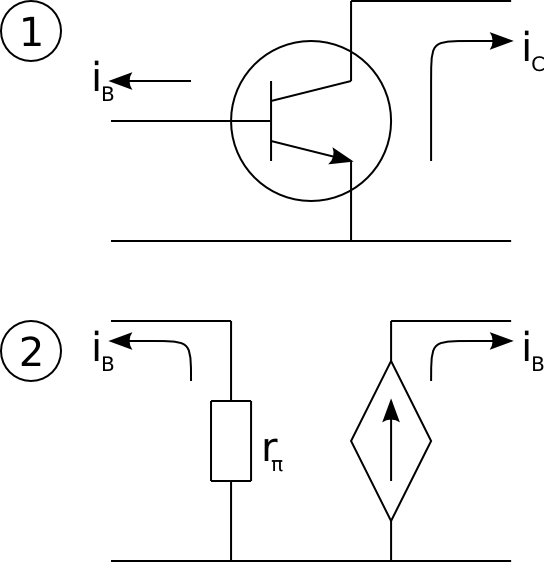
\includegraphics[width=0.5\textwidth]{./img/smasignal}
\\\\
$$i_C = \beta \cdot i_B$$
$$i_C = g_m \cdot V_{BE}$$

\subsubsection{Steilhet}
Transkonduktans?
TODO

\subsubsection{Dynamisk inngangsresistans}
TODO
